\chapter{Repository Deep Dive}\label{chap:Repository_Deep_Dive}
In this section, we lightly discuss each of the subdirectories present within the root of Chipyard, take note of any particularly important files, and demonstrate how this entire system is put together.

\section{Languages Used in Chipyard}\label{sec:Langs_used_in_Chipyard}
There are several programming languages used in the construction of Chipyard that you should be at least familiar with.
They are:
\begin{itemize}
\item \href{https://www.gnu.org/software/make/}{Make}.
  Discussed in \Cref{sec:Makefiles_in_Chipyard}
\item \href{https://www.scala-lang.org/}{Scala}
\item \href{https://www.chisel-lang.org/}{Chisel}/\Gls{firrtl}.
  Both of these are programs that work using files written in Scala \glspl{dsl}.
\item \href{https://en.wikipedia.org/wiki/Verilog}{Verilog}
\end{itemize}

In short, Make and its Makefiles are used to glue all the separate parts of the Chipyard framework together.
By calling a single \texttt{make} command, and possibly providing flags, all the necessary dependencies are found locally, and placed in the right search locations.
It also handles the process of directing \gls{sbt} to work on the proper files.

Each of the generators and Chipyard itself parameterizes the Verilog code using Scala.
Verilog is the lowest-level ``programming language'' used in this framework.
It defines the semantic behavior of circuits.
Scala is then used to allow multiple of the same Verilog module to be used in parallel, or composed in other, more exotic ways.

The most direct example of this is the use of Scala to parameterize the number of Rocket cores to include in the generated CPU design.
\Cref{lst:Scala_Parameterized_Verilog} is a good example of this.

\begin{listing}[h!tbp]
\begin{minted}[frame=lines,linenos]{scala}
class QuadRocketConfig extends Config(
    new freechips.rocketchip.subsystem.WithNBigCores(4) ++
    new chipyard.config.AbstractConfig)
\end{minted}
\caption{Example of Scala-Parameterized Verilog}
\label{lst:Scala_Parameterized_Verilog}
\end{listing}

In \Cref{lst:Scala_Parameterized_Verilog}, the method \texttt{WithNBigCores} will return a class of big \nameref{sec:Rocket_Chip} cores.
By providing an integer to the class constructor, that many core objects are returned.
This informs \gls{firrtl} about the proper system setup, so that it can elaborate the design, creating the final product.
If someone wanted eight, twelve, or even thirty-two cores, they simply have to change the passed integer, and have a hosting system that has enough resources to elaborate such a complicated design.
This eases the Verilog writer's job as well, because they only need to write their hardware description module for a single CPU, and they do not need to worry about multiple processors.

\section{Makefiles, or the Glue of this Framework}\label{sec:Makefiles_in_Chipyard}
Chipyard makes \textbf{heavy} use of Makefiles to pull together and automate various parts of the build system.
Variables and/or values that are shared between different ways of building systems are higher in the directory structure.

Thus, some of the most overarching commands and variables for this project are defined in \file{chipyard/variables.mk}.
One of the first things defined within this file are numerous output messages.

\subsection{\texttt{SUB\_PROJECT}}\label{subsec:Makefile_SUB_PROJECT}
The first notable part of the \file{variables.mk} file is the \texttt{SUB\_PROJECT} defaulting variable.
This particular variable is what allows for easy re-configuration of the entire framework to support elaborating your own CPU designs.
By changing this file between one of the well-defined options, one can easily re-use major portions of Chipyard's architecture.

For example, to switch from a CPU defined by Chipyard to one that is uses the Hwacha accelerator, one just needs to say \mintinline{bash}{make SUB_PROJCT=hwacha}, and all the necessary configuration variables are changed.

\subsection{Building Each Subproject}\label{subsec:Building_Each_Subproject}
The next notable part of this file is its large \mintinline{make}{ifeq ... endif} blocks.
Each one of these defines a different subproject that can be built and elaborated upon by Chipyard and its surrounding framework.
These subproject defining blocks each define multiple higher-level variables which are the variables that are actually used to build and test each of the CPUs.
Each of the variables is important, and Chipyard provided documentation for each variable inside \file{variables.mk}.
However, additional information that we gathered through trial-and-error is presented below.

\begin{description}
\item[\texttt{SUB\_PROJECT}] This corresponds to one of the projects in the \file{chipyard/generators} directory.
  More formally, it is defined by one of the entries in the \file{build.sbt} files in the respective generators directory, and by the main \file{build.sbt} file in the root of Chipyard.
\item[\texttt{SBT\_PROJECT}] This corresponds to a top-level of the repository of the chip to build.
  This is where many of the higher-level constructs, such as the test harness and test bench are defined from.
\item[\texttt{MODEL}] The model is the top-level module of the project that should be used by Chisel.
  Normally, this should be defined to the be same as the test harness, but does not necessarily have to be.
\item[\texttt{VLOG\_MODEL}] This is the top-level module of the project that should be used by FIRRTL/Verilog.
  Like \texttt{MODEL}, this is usually the same as the test harness, but does not necessarily need to be.
\item[\texttt{MODEL\_PACKAGE}] This is the Scala package that is used to find the overall model of the CPU.\@
  This should correspond to the \mintinline{scala}{package <packageName>} in a Scala CPU configuration file.
\item[\texttt{CONFIG}] This defines the parameters that should be used for the project.
  Typically, this is used to select one of the CPU configurations defined in the \texttt{SBT\_PROJECT}.
\item[\texttt{CONFIG\_PACKAGE}] This is the Scala package that defines the \texttt{Config} class.
  This file \textbf{MUST} contain the class definition for \texttt{Config}, meaning \mintinline{scala}{object Config} must be present.
\item[\texttt{GENERATOR\_PACKAGE}] This is the Scala package that defines the \texttt{Generator} class.
  This file \textbf{MUST} contain the class definition for \texttt{Generator}, meaning \mintinline{scala}{object Generator} must be present.
\item[\texttt{TB}] This defines the test bench wrapper that extends over the test harness to allow for simulation in a Verilog simulator.
\item[\texttt{TOP}] This is the top-level module of the project.
  Typically, this is the module instantiated by the test harness.
\end{description}

\section{\file{build.sbt}}\label{sec:build.sbt}
There are two main \file{build.sbt} files that you should be aware of.
There is a \file{build.sbt} for each of the generator subdirectories.
These define some metadata information about each of the projects, such as the name of the design, the authors of the design, the targeted \texttt{sbt} version, and others.

However, the \file{build.sbt} file in the root of Chipyard is a metadata file not just for Chipyard itself, but also pulls together all the dependencies in \file{chipyard/generators/} so that they all can be elaborated upon with Chipyard.

% TODO: Rework this paragraph about circular dependency in main build.sbt file.
This file is also the one that should be used for defining your \emph{own} CPU.\@
Note that this means you are building your own Verilog code which defines the generation rules for a CPU.\@
However, one must be careful that they do not introduce circular dependencies into the dependency graph between the CPU generation and elaboration tools.
Even though Scala has support for lazy evaluation, it does not completely extend to dependency evaluation, and the entire system can fall apart.
This does \emph{not} mean that you use this to build a new CPU on top of the architecture already defined by Chipyard, or any other CPU.\@
However, you can use other CPU-generating systems inside your design.

\subsection{About}\label{sec:About_Verilator_Simulator}
The primary way to simulate SoCs' designed using the Chipyard framework is via Verilator simulations.
The directory for verilator is \file{chipyard/sims/verilator}.
An example simulation can be run by using \mintinline{bash}{make} in the verilator directory.
Running the \texttt{make} command produces a simulator executable in the verilator directory.

Custom Chipyard configs can be simulated by running \mintinline{bash}{make CONFIG=<your custom config>}.
For example, if your project name was ``TestConfig'', running \mintinline{bash}{make CONFIG=TestConfig} would create an executable called \file{simulator-chipyard-TestConfig} in the \file{verilator} directory.
Custom RISCV code can be run by using the command \mintinline{bash}{./simulator-chipyard-TestConfig /path/to/riscv/executable} from the \file{chipyard/sims/verilator} directory.

\section{Generators}\label{sec:Generators}
In this section, we look at each of the subdirectories inside the \file{chipyard/generators} subdirectory in turn.
Each of the CPU generators presented below are each slightly unique in their implementation of the open RISC-V ISA.\@

\subsection{BOOM}\label{sec:BOOM_Generator}
\nocite{boomHomepage}
\nocite{boomGithub}
\nocite{boomPaper}
BOOM~(Berkeley Out-of-Order Machine) is a CPU defined and built by Univerity of California at Berkeley that implements the RISC-V Instruction Set Architecture (ISA).
Its claim to fame is that it can execute RISC-V instructions out-of-order, thereby drastically improving performance.
It is designed to be highly performant, synthesizable, and parameterizable.

BOOM includes support for the following operations:
\begin{itemize}
\item Floating Point (IEEE 754--2008)
\item Atomic Operations
\item Caching
\item Virtual Memory
\end{itemize}
In addition, BOOM supports external debugging.
Microarchitectural documentation can be found \href{https://docs.boom-core.org/en/latest/}{here}.
The GitHub organization and its development can be found \href{https://github.com/riscv-boom}{here}.

These CPU definitions are used by \nameref{sec:Chipyard_Generator} when elaborating CPU designs defined by the end-programmer.

\subsection{Chipyard}\label{sec:Chipyard_Generator}
This is the main source of truth inside this repository.
Here is where all of the code required to get these disparate CPUs to work and build together is located.
Typically, very little editing is needed to be done here.
Most of the editing in this repository comes in the form of defining your own CPUs, which are themselves defined in terms of other CPUs or other lower-level Chipyard constructs.

The main point of interest is the \file{chipyard/generators/chipyard/src/main/scala/config} directory.
This houses CPU design configuration files written in Scala.
Each of them defines a different class of CPU, ranging from \nameref{sec:BOOM_Generator} to \nameref{sec:cva6_Generator}, to \nameref{sec:RISC-V_Sodor} configurations.
Each design is a class described in each one of these files.

\subsection{cva6}\label{sec:cva6_Generator}
\nocite{cva6Github}
\nocite{zaruba2019cost}
cva6 is a 6-stage, single issue, in-order CPU.\@
This means that unlike the \nameref{sec:BOOM_Generator} design, instructions are \emph{always} executed in order.
It fully implements the 64-bit RISC-V instruction set, and several extensions, including:
\begin{description}
\item[I] Base Integer (the base 64-bit instruction set)
\item[M] Integer Multiplication and Division
\item[A] Atomic Operations
\item[C] Compression/Decompression Operations
\end{description}
In addition, it supports three different privilege levels, M, S, and U.
This allows the chip to run a full Unix-like operating system.

\subsection{Gemmini}\label{sec:Gemmini_Generator}
\nocite{gemminiGithub}
\nocite{gemminiPaper}
Gemmini is not a CPU;\@ instead, it is a CPU \emph{accelerator}, implemented alongside another CPU, such as a \nameref{sec:BOOM_Generator} or \nameref{sec:Rocket_Chip} design.
It is intended for hardware-level matrix operations, such as matrix multiplication, machine learning, and other \gls{simd} operations.
A general logic design for the Gemmini accelerators is shown in \Cref{fig:Gemmini_Accelerator}.

\begin{figure}[h!tbp]
  \centering
  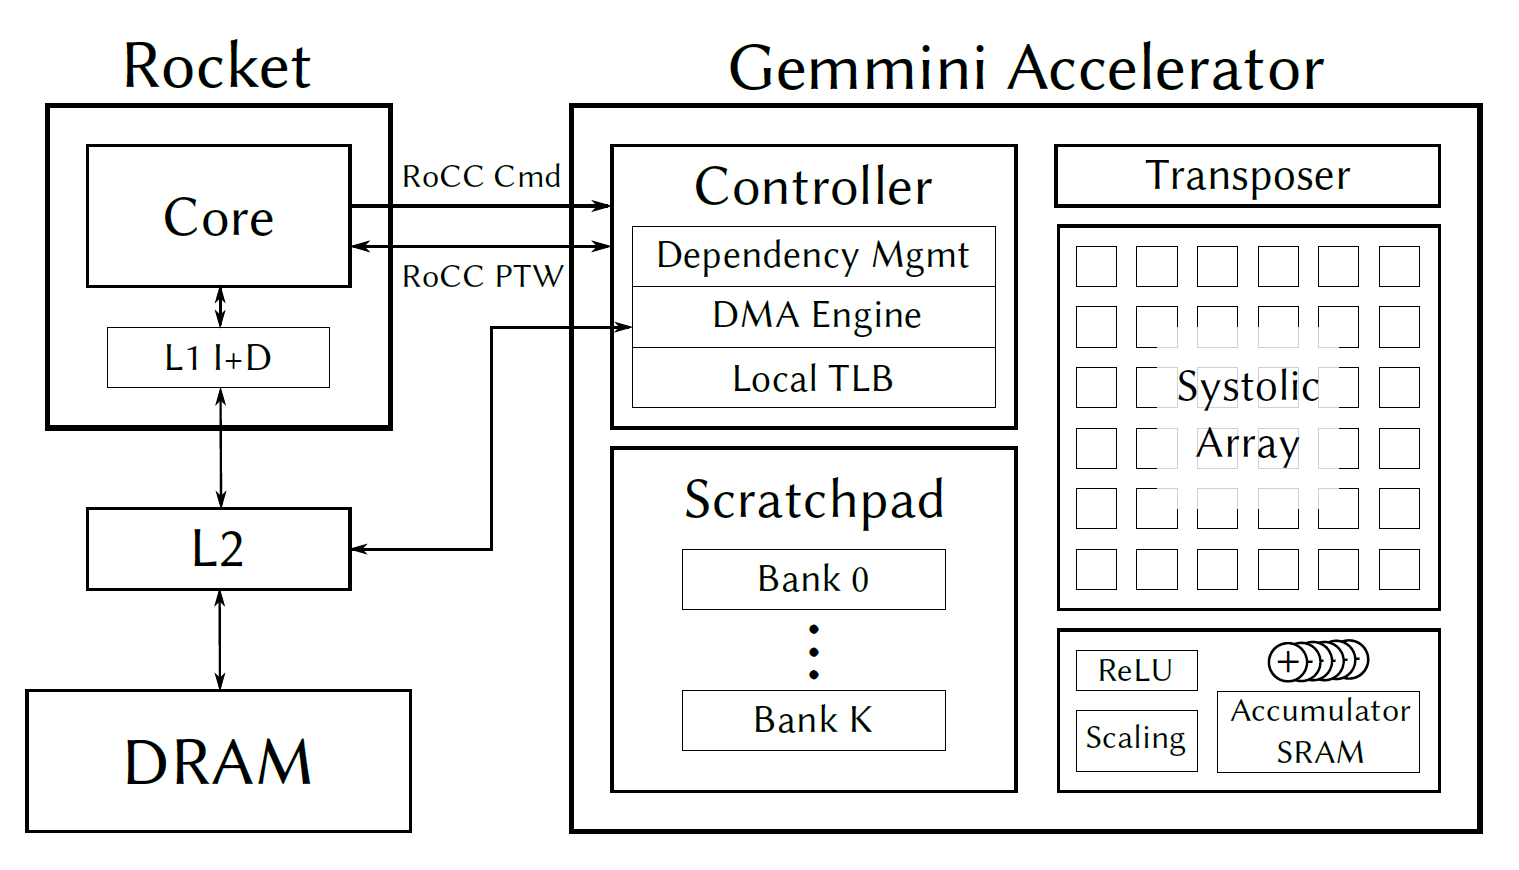
\includegraphics[scale=0.55]{./gemmini-system.png}
  \caption{Gemmini Accelerator Logic Design \parencite{gemminiGithub}}
  \label{fig:Gemmini_Accelerator}
\end{figure}

Gemmini is intended for integration with other \nameref{sec:Rocket_Chip}s, but can be configured to work with \nameref{sec:BOOM_Generator} chips as well.

\subsection{Hwacha}\label{sec:Hwacha}
\nocite{hwachaGithub}
\nocite{hwachaPresentation}
Like the \nameref{sec:Gemmini_Generator}, Hwacha is meant to be an accelerator.
Hwacha is a co-processor, designed to be run with other CPU processors, namely the \nameref{sec:Rocket_Chip}s.
Hwacha, like \nameref{sec:Gemmini_Generator}, is another \gls{simd} co-processor, but designed to work with vectors instead or matrices.

It uses several alternative concepts in its design, including:
\begin{itemize}
\item A configurable register file, which is defined by software
\item A runtime-variable vector length register
\item Aggressive prefetching of memory, due to constant-stride memory accesses
\item Resolving memory references as early as possible.
\item Along with several others
\end{itemize}

These all feed into Hwacha's goal of maximizing the efficiency of an in-order vector microarchitecture.
It was designed to be usable with another CPU to run an operating system that supports unified virtual memory and restartable exceptions.
A block-level diagram of the major components in the Hwacha coprocessor is shown in \Cref{fig:Hwacha_Accelerator}

\begin{figure}[h!tbp]
  \centering
  % TODO: Recreate as vector image?
  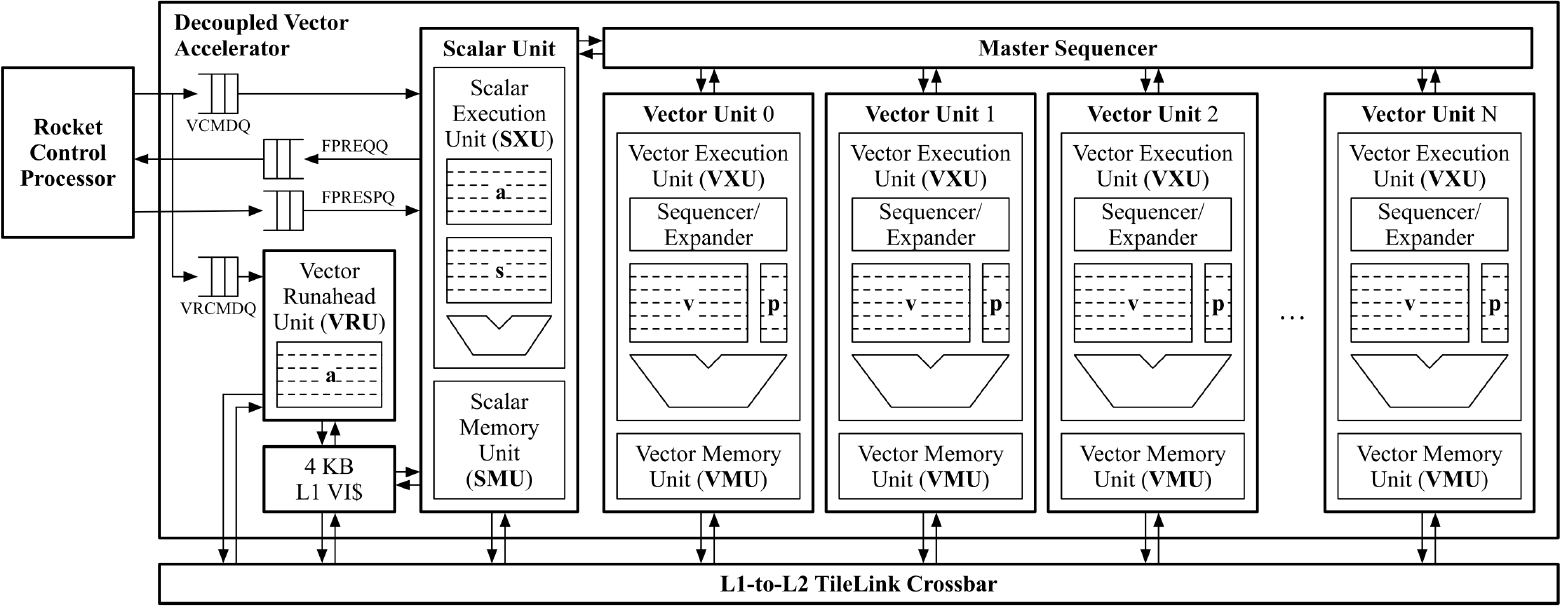
\includegraphics[scale=0.42]{./hwacha-system.png}
  \caption{Hwacha Design~\cite[p.~11]{hwachaPresentation}}
  \label{fig:Hwacha_Accelerator}
\end{figure}

\subsection{Icenet}\label{sec:Icenet_Generator}
\nocite{icenetGithub}
Icenet is a generator that is no less interesting, but less applicable to our uses.
It is intended to provide Ethernet-based networking components in support of the \nameref{sec:FireSim_Simulator} design simulator.
Like all other components in Chipyard, this is also parameterizable, allowing for multiple \Glspl{nic} to be defined.
Because we were more focused on getting generated RISC-V images written to an \Gls{fpga} for local testing, we did not investigate this particular generator.
The overall design of Icenet is shown in \Cref{fig:Icenet_Generator}.

\begin{figure}[h!tbp]
  \centering
  % TODO: Recreate with vector graphics. The Rasterized PNG is terrible.
  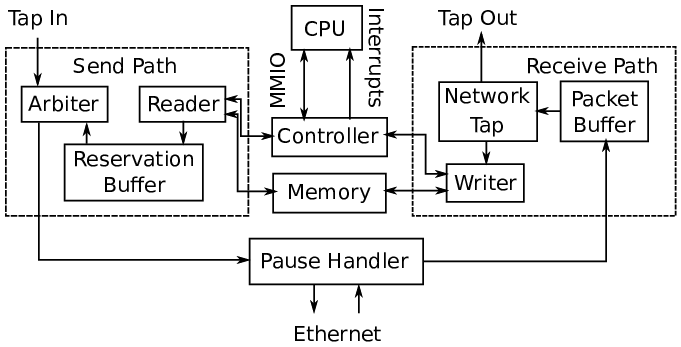
\includegraphics[scale=0.50]{./icenet-design.png}
  \caption{Icenet Design}
  \label{fig:Icenet_Generator}
\end{figure}

Icenet's controller works by exposing a set of \gls{mmio} registers to the CPU.\@
These registers define where in memory to read data from/write data to.
The design also has a reservation queue buffer so that TileLink responses that come out of order are provided to the CPU in the proper order.
Icenet also provides a kernel driver so that the \gls{nic} has a full Linux networking stack in userspace.

\subsection{NVDLA}\label{sec:NVDLA_Generator}
\nocite{nvdlaPaper}
\nocite{nvdlaNVIDIAPresentation}
NVDLA, short for NVIDIA Deep Learning Accelerator, is a domain-specific \gls{soc}, designed specifically for deep learning.
It is optimized for deep learning tasks, such as Convolutional Neural Networks and computer vision.
It is targeted for edge-computing devices, primarily for \Gls{iot}.
This particular \gls{soc} design was \emph{not} investigated, as it is both proprietary and outside the scope of this particular research.

\subsection{RISC-V Sodor}\label{sec:RISC-V_Sodor}
\nocite{sodorGithub}
Sodor is actually a collection of several different simple integer pipelines for RISC-V.
Each one of these implementes the full RISC-V 32b user-level integer base (RV32I).
\textbf{None} of the cores support virtual memory, and all of them interace with a simple asynchronous single-cycle block of memory.

There are five different pipelines:
\begin{description}
\item[1-Stage] An \gls{isa} simulator.
\item[2-Stage] Demonstrates pipelining in Chisel.
\item[3-Stage] Uses sequential memory, supporting both Harvard and Princeton CPU architectures.
\item[5-Stage] Toggle between bypassed or interlocked memory.
\item[Bus-Based] A CPU based around a central bus.
\end{description}

This particular set of cores would be most applicable for courses in computer architecture, as the cores are relatively simple and easy to modify.
In addition, the \href{https://github.com/ucb-bar/riscv-sodor}{repository} for these cores also already includes undergraduate laboratory materials.

\subsection{Rocket-Chip}\label{sec:Rocket_Chip}
\nocite{rocketChipPaper}
\nocite{rocketChipGithub}
Rocket Chip is a \gls{soc} design generator that outputs synthesizable \gls{rtl}.
This allows for this \gls{soc} to be composed of computer-generated cores, caches, and interconnects.
The Rocket Chip is a general-purpose processor core that uses the RISC-V \gls{isa}, and includes support for virtual memory.
It is a superset of the \nameref{sec:BOOM_Generator}, because it provides both an in-order execution core generator (Rocket), and the specialized \nameref{sec:BOOM_Generator} configuration for out-of-order execution.

What makes Rocket different than other chips is that it can be used to create larger heterogenous \glspl{soc}.
This means that a single package can be composed of not only Rocket CPUs, but \emph{also} custom acclerators, co-processors, or completely independent cores, or even a mix of all three.

Overall, the Rocket chip is an \gls{soc} design that is most useful for general-purpose computing platforms and CPU and \gls{fpga} research.
Its open development platform and extensible design allows for anyone to use the already defined designs and extend on top of them.
The Rocket Chip design is the paragon of RISC-V extensibility due to its support for adding additional processing units on-board that perform tasks in hardware rather than software.

\subsection{SHA3}\label{sec:SHA3_Accelerators_Generator}
\nocite{sha3Paper}
\nocite{sha3Github}
The SHA3 generator is a parameterized accelerator compute unit, like the \nameref{sec:Gemmini_Generator} and \nameref{sec:Hwacha}.
As it is parameterized, its overall characteristics and funtionality can change based on the input parameters to the design system.
It was designed to be an example of making an add-on computational unit for the \nameref{sec:Rocket_Chip} and \nameref{sec:BOOM_Generator} cores.
The overall design of the accelerator is given in \Cref{fig:SHA3_Accelerator_Design}, drawn from~\cite{sha3Paper} and fetched from~\cite{sha3Github}.

\begin{figure}[h!tbp]
  \centering
  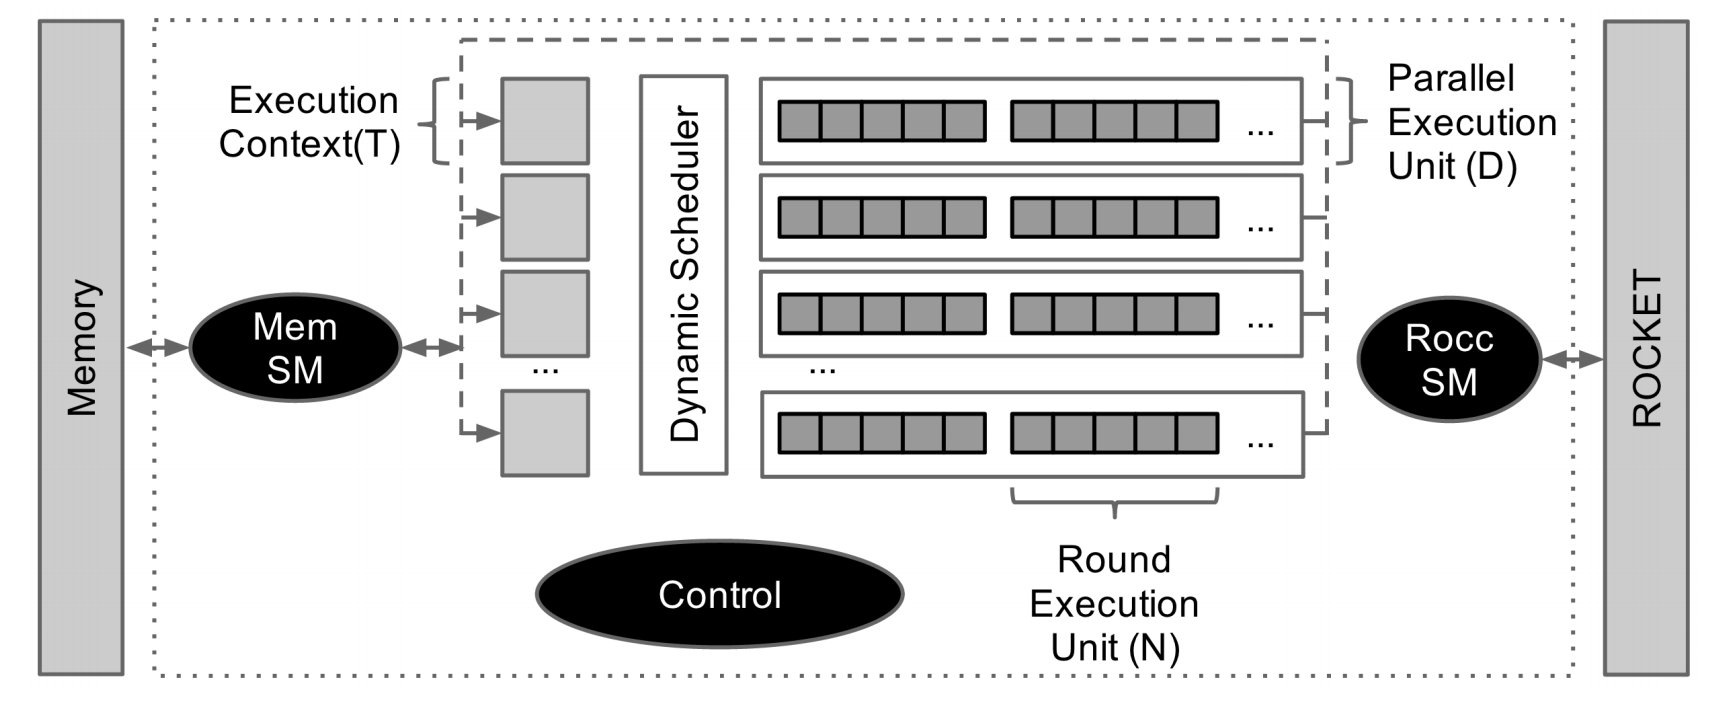
\includegraphics[scale=0.25]{./sha3-system.png}
  \caption{SHA3 Accelerator Design~\cite[p.~3]{sha3Paper}}
  \label{fig:SHA3_Accelerator_Design}
\end{figure}

The design is a fully featured SHA3 computing unit that has the ability to be given the memory address whose contents are to be hashed, the computation to perform, and the memory location where to store the result.
All of this is done in a ``set and forget'' kind of way, where the main processor gives the accelerator the required information and the accelerator is free to run on its own.

To add a SHA3 accelerator to your \nameref{sec:Rocket_Chip} or \nameref{sec:BOOM_Generator} design, follow the example code shown in \Cref{lst:SHA3_Accelerator_Addition}.

\begin{listing}[h!tbp]
\scalasourcefile{./code/add-sha3-accelerator.scala}
\caption{Add SHA3 Accelerator to Rocket Design}
\label{lst:SHA3_Accelerator_Addition}
\end{listing}

\subsection{SiFive Blocks}\label{sec:SiFive_Blocks}
\nocite{siFiveBlocksGithub}
This generator is mainly intended to be used a building block for other, higher-level, modules.
It defines many common \gls{rtl} blocks that are typically used for SiFive's other projects.
Because Chipyard requires integration with many other technologies, they also rely on the code that is already defined in the \texttt{sifive-blocks} repository.

\subsection{SiFive Cache}\label{sec:SiFive_Cache}
\nocite{siFiveCacheGithub}
Like \nameref{sec:SiFive_Blocks}, SiFive's cache is intended to be used to build higher-level modules.
It defines the necessary terms to paramterize and generate the required \gls{rtl} to create a last-level inclusive cache.
Cache coherence is enforced using an invalidation policy.
SiFive Cache is intended to be a drop-in replacement for \nameref{sec:Rocket_Chip}'s \texttt{tilelink.BroadcastHub} coherence manager.

\subsection{\file{testchipip}}\label{sec:testchipip}
\nocite{testchipipGithub}
This last generator module is used to integrate proprietary intellectual property~(IP) components with the rest of the generated system.
It provides:
\begin{enumerate}
\item Clock utilities
\item Utilities to interface SERDES to and from TileLink
\item Custom serial interfaces for debugging with simulator interface
\item TileLink splitter, switcher
\item Several other components
\end{enumerate}

\section{Custom Configurations}\label{sec:Custom_Configurations}
When defining a custom configuration that is based on the work already done in Chipyard, and you want to pull in the all the other work from all other generators, the new configuration class \textbf{must} be defined in the \file{chipyard/generators/chipyard/src/main/scala/config/} directory.

\begin{blackbox}
  Note that this case is distinctly different than when you define your own custom parameterized \gls{rtl} Verilog to generate \textbf{new} modules.
  In the case you are defining a new processor design, but you want to continue building off the work of the code that is already defined, you \textbf{must} place your custom class in Chipyard's \file{config/} directory.

  In the case you are defining a completely new design (a new accelerator for instance), you can separate this definition out to a different generator directory entirely.
  Then, you can track that as a submodule of Chipyard, have Chipyard import, and dynamically handle your new project as a dependency of the one that generates the CPU design.
\end{blackbox}

In this section, we show how to create a new, custom, configuration that combines the already-existing projects.
We will be building a processor using four medium-sized \nameref{sec:Rocket_Chip} general-purpose cores, the default memory configuration, and will attach a SHA3 accelerator to the design for hardware-accelerated SHA3 calculation.

We will cover how to write a generated design image out to an \gls{fpga} in \Cref{chap:FPGA_Implementation}, rather than here, because the process is the same for every generated chip.

\subsection{File and Class Creation}\label{sec:Custom_Config-File_Class}
Start by creating the \file{NewTestConfig.scala} file in the \file{chipyard/generators/chipyard/src/main/scala/config/} directory.
Inside of this file, we will start defining the \texttt{NewTestConfig} class, which will declare the desired configuration.

\begin{blackbox}
  Example configurations of various homogenous and heterogenous chips can be found in \file{RocketConfigs.scala}, in the same directory.
\end{blackbox}

We want our processor design to be quite simple, so we are designing a processor that uses only in-order execution.
In addition, we want to design a processor that has multiple cores on it,because a single CPU design for general-purpose use is not enough today.
Lastly, we want to include a \nameref{sec:SHA3_Accelerators_Generator} accelerator module to allow us to perform SHA3 computations in hardware.

In short, our design will have:
\begin{enumerate}
\item Multiple \nameref{sec:Rocket_Chip} cores.
  We are going to start with four medium-sized cores.
  There are both larger and smaller sizes already defined.
\item A single \nameref{sec:SHA3_Accelerators_Generator} accelerator.
\end{enumerate}

Using the design parameters we have defined, we can write a processor definition class that \emph{declaratively} describes the resulting CPU we want.
The code for this is shown in \Cref{lst:Custom_Config-NewTestConfig} and is also available alongside the source code for this document.

\begin{listing}[h!tbp]
\scalasourcefile{./code/NewTestConfig.scala}
\caption{\file{NewTestConfig.scala} Contents}
\label{lst:Custom_Config-NewTestConfig}
\end{listing}

\subsection{Building}\label{sec:Custom_Config-Building}

\subsection{Testing}\label{sec:Custom_Config-Testing}

\subsection{Simulating}\label{sec:Custom_Config-Simulating}

%%% Local Variables:
%%% mode: latex
%%% TeX-master: "../doc"
%%% End:
